\documentclass[11pt,a4paper,twoside,fleqn]{article}
\usepackage[utf8]{inputenc}
\usepackage[german]{babel}
\usepackage[left=25mm, top=20mm, bottom=20mm, right=20mm]{geometry}
\usepackage{graphicx,color,marvosym,upgreek}
\usepackage{amssymb,multicol,overpic}
\usepackage{amsmath, enumitem}
% \usepackage{ifthen}

%% http://www.ctan.org/pkg/exsheets
\usepackage[totoc=false]{exsheets}


\begin{document}

\renewcommand{\thepage}{Seite~\arabic{page}}
% \renewcommand{\thesection}{1.}
% \renewcommand{\thesubsection}{\arabic{subsection}}
\renewcommand{\baselinestretch}{1.2}

\renewcommand{\labelenumi}{{\bf\arabic{enumi}.)}}
\renewcommand{\labelenumii}{{\bf\alph{enumii})}}
\renewcommand{\labelenumiii}{{\bf\roman{enumiii})}}

\newcounter{column}
\renewcommand{\thecolumn}{{\bf\alph{column}\ }}
\newcommand{\labelcolumn}{{\bf\alph{column})\ \ \ }}
\setlength{\itemsep}{0pt}
\setlength{\mathindent}{0cm}
\newcounter{last}


\SetupExSheets{question/headings=runin,question/type=exam}



\pagestyle{myheadings}
\markboth{\hfill Kurs: Funktionenscharen}%
{Kurs: Funktionenscharen\hfill}
\title{Funktionenscharen\\\large{Ein Kurs
    zum selbständigen Lernen}}
\author{Alexander Ruhri\\
  \small\texttt{a.ruhri@widarschule.de}\\
  \small Aktuelle Version unter \texttt{http://www.ruhri.net/}
}
\date{\small Version 0.1, September 2014}

\maketitle
\section*{Vorbemerkungen}
Bitte beachten Sie beim Bearbeiten dieser Blätter, dass an geeigneten
Stellen Zusammenfassungen mit der ganzen Klasse durchgeführt
werden. Bitte machen Sie Ihren Lehrer darauf aufmerksam, wenn Sie das
Bedürfnis nach einer solchen Besprechung haben. 

Besonders wichtig ist das Notieren der wichtigsten Ergebnisse in ein
Regelheft. Vergleichen Sie diese Regeln bzw. besprechen Sie sie mit
der ganzen Klasse, damit Sie sicher sein können, dass sie korrekt sind.

\subsection*{Voraussetzungen}
Um diesen Kurs erfolgreich absolvieren zu können, ist es notwendig,
dass Sie mit ganzrationalen Funktionen vertraut sind. Sie sollten mit
der Untersuchung von Funktionen (Nullstellen, Extrema, Wendepunkte)
und der Integralrechnung vertraut sein. 

\tableofcontents

\section{Scharen von Funktionen}
In vielen Sachzusammenhängen, die durch eine ganzrationale Funktion
beschrieben werden, kann es sinnvoll sein sich verändernde Parameter
in den Funktionsterm aufzunehmen, damit man nicht für jede neue
Situation eine neue Funktion braucht, sondern einfach nur den
Parameter anpassen muss.

Dadurch entstehen unter Umständen unendliche viele Funktionen (für
jeden möglichen Parameter eine) die zusammen gehören. Mit dem Begriff
„Schar“ wird diese Zusammengehörigkeit zum Ausdruck gebracht.

\subsection{Das Schachtelproblem}
\noindent\begin{minipage}[t]{.75\linewidth}
  Wir betrachten unser bekanntes „Schachtelproblem“, bei dem eine
  Schachtel aus einem quadratischen Stück Pappe gefaltet wird, indem
  man in den Ecken Quadrate der Seitenlänge $x$ ausschneidet. Je nach
  Wahl von $x$ hat die Schachtel ein anderes Volumen.
\end{minipage}\hfill
\begin{minipage}[t]{.2\linewidth}
  \vspace{-3\baselineskip}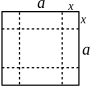
\includegraphics[width=\linewidth]{pics/1_schachtel_1}
\end{minipage}

\begin{question}%[type=exam]
  \begin{enumerate}
  \item Bestimmen Sie den Funktionsterm\footnote{Der Funktionsterm ist
    der Term „$x^3-4x$“ in der Funktionsgleichung $f(x)=x^3-4x$, also
    in der Regel die rechte Seite der Funktionsgleichung.} des Volumens $V(x)$ einer Schachtel aus
    einer Pappe mit Kantenlänge $a$ in Abhängigkeit von $x$.
    \begin{multicols}{3}
      \begin{enumerate}
      \item $a=30\,$cm
      \item $a=60\,$cm
      \item $a=90\,$cm
      \end{enumerate}
    \end{multicols}
  \item Welche Werte darf denn das $x$ annehmen, damit die
    mathematische Beschreibung im Sachzusammenhang Sinn macht?
  \item Bestimmen Sie für jede Schachtel aus der vorigen Aufgabe das
    $x$, bei dem das Volumen der Schachtel maximal ist.
  \item \label{regel1}Notieren Sie die Regelmäßigkeit, die Sie dabei feststellen konnten.
  \end{enumerate}

  Zur Vereinfachung, damit man nicht für jede neue Pappe eine neue
  Funktion braucht, kann die Kantenlänge der Pappe unbestimmt gelassen 
  werden und als Parameter $a$ in den Funktionsterm eingeführt werden.
  \begin{enumerate}[resume]
  \item Bestimmen Sie den Funktionsterm des Volumens $V_a(x)$ einer
    Schachtel aus einer Pappe mit beliebiger Kantenlänge $a$.

    Das $a$
    im Index des Funktionsnamens weist darauf hin, dass der
    Funktionsterm von einem Parameter abhängig ist. Für $a$ gilt
    natürlich: $a > 0 $ und $a \in\mathbb{R}$ oder kurz:
    $a\in\mathbb{R}^+$, weil es eine Seitenlänge ist und somit nur
    positive Werte annehmen kann.
  \item Zeichnen Sie die Graphen von $V$ für die Seitenlängen
    $a=75\,$cm, $a=60\,$cm und $a=45\,$cm in \emph{ein}
    passendes\footnote{Tipp: $0 \leq x \leq 40$ und $0 \leq y \leq 32000$}
    Koordinatensystem. 
  \item Bestimmen Sie nun das Maximum\footnote{Zur Erinnerung: Das
      Maximum ist ein Punkt. Zur Erinnerung: Ein Punkt hat immer zwei
      Koordinaten.} der Volumensfunktion für jede 
    Schachtel aus einer Pappe der Seitenlänge $a$. Beachten Sie beim
    Ableiten, dass $a$ eine fest gewählte Zahl 
    ist, nämlich die Seitenlänge der Pappe, denn die muss ja vorher
    festgelegt sein.
  \item Vergleichen Sie das Ergebnis mit der gefundenen Regelmäßigkeit
    aus Aufgabe \ref{regel1}.).
  \end{enumerate}
\end{question}
\begin{solution}  
  \begin{enumerate}
  \item 
    \begin{multicols}{2}
      \begin{enumerate}
      \item $V(x)=x\cdot (30-2x)^2=\\4x^3-120x^2+900x$
      \item $V(x)=4x^3 - 240x^2 +3600x$
      \item $V(x)=4x^3 - 360x^2 + 8100x$
      \end{enumerate}
    \end{multicols}
  \item Das $x$ muss größer als $0$ sein, darf aber nicht größer als
   die halbe Seitenlänge der Pappe sein. (Begründen Sie!)
  \item 
    \begin{enumerate}
   
        \item $V^\prime(x)=12x^2-240x +900$ und
        $V^{\prime\prime}(x)=24x -240$

        $V^\prime(x)=0 \Leftrightarrow x=15 \vee x=5$ Für $x=15$ ist
        das Volumen null (warum?), $V^{\prime\prime}(5)=-120 < 0$, also
        erhält man das maximale Volumen der Schachtel, wenn man ein
        Quadrat der Seitenlänge $x_{max}=5$ ausschneidet.
        \begin{multicols}{2}
        \item $x_{max}=10$
        \item $x_{max}=15$
  
      \end{multicols}
        \end{enumerate}
  
      \item Vergleichen Sie mit Ihren Klassenkollegen!
      \item Das Volumen jeder Schachtel kann dann einfach durch
        $V_a(x)=x\cdot (a - 2x)^2$ ausgedrückt werden.  Durch Anwenden
        der binomischen Formel erhalten wir $ V_a(x)=x\cdot(a^2 - 4ax
        + 4x^2)$ und weiter: $ V_a(x)=4x^3 - 4ax^2+ a^2x$, wobei
        natürlich wegen des Sachzusammenhangs gilt: $0 < x < \frac a
        2$ und $a\in\mathbb{R}^+$.
      \item 
        Für ein fest gewähltes $a$ wird jeweils ein Graph gezeichnet.

        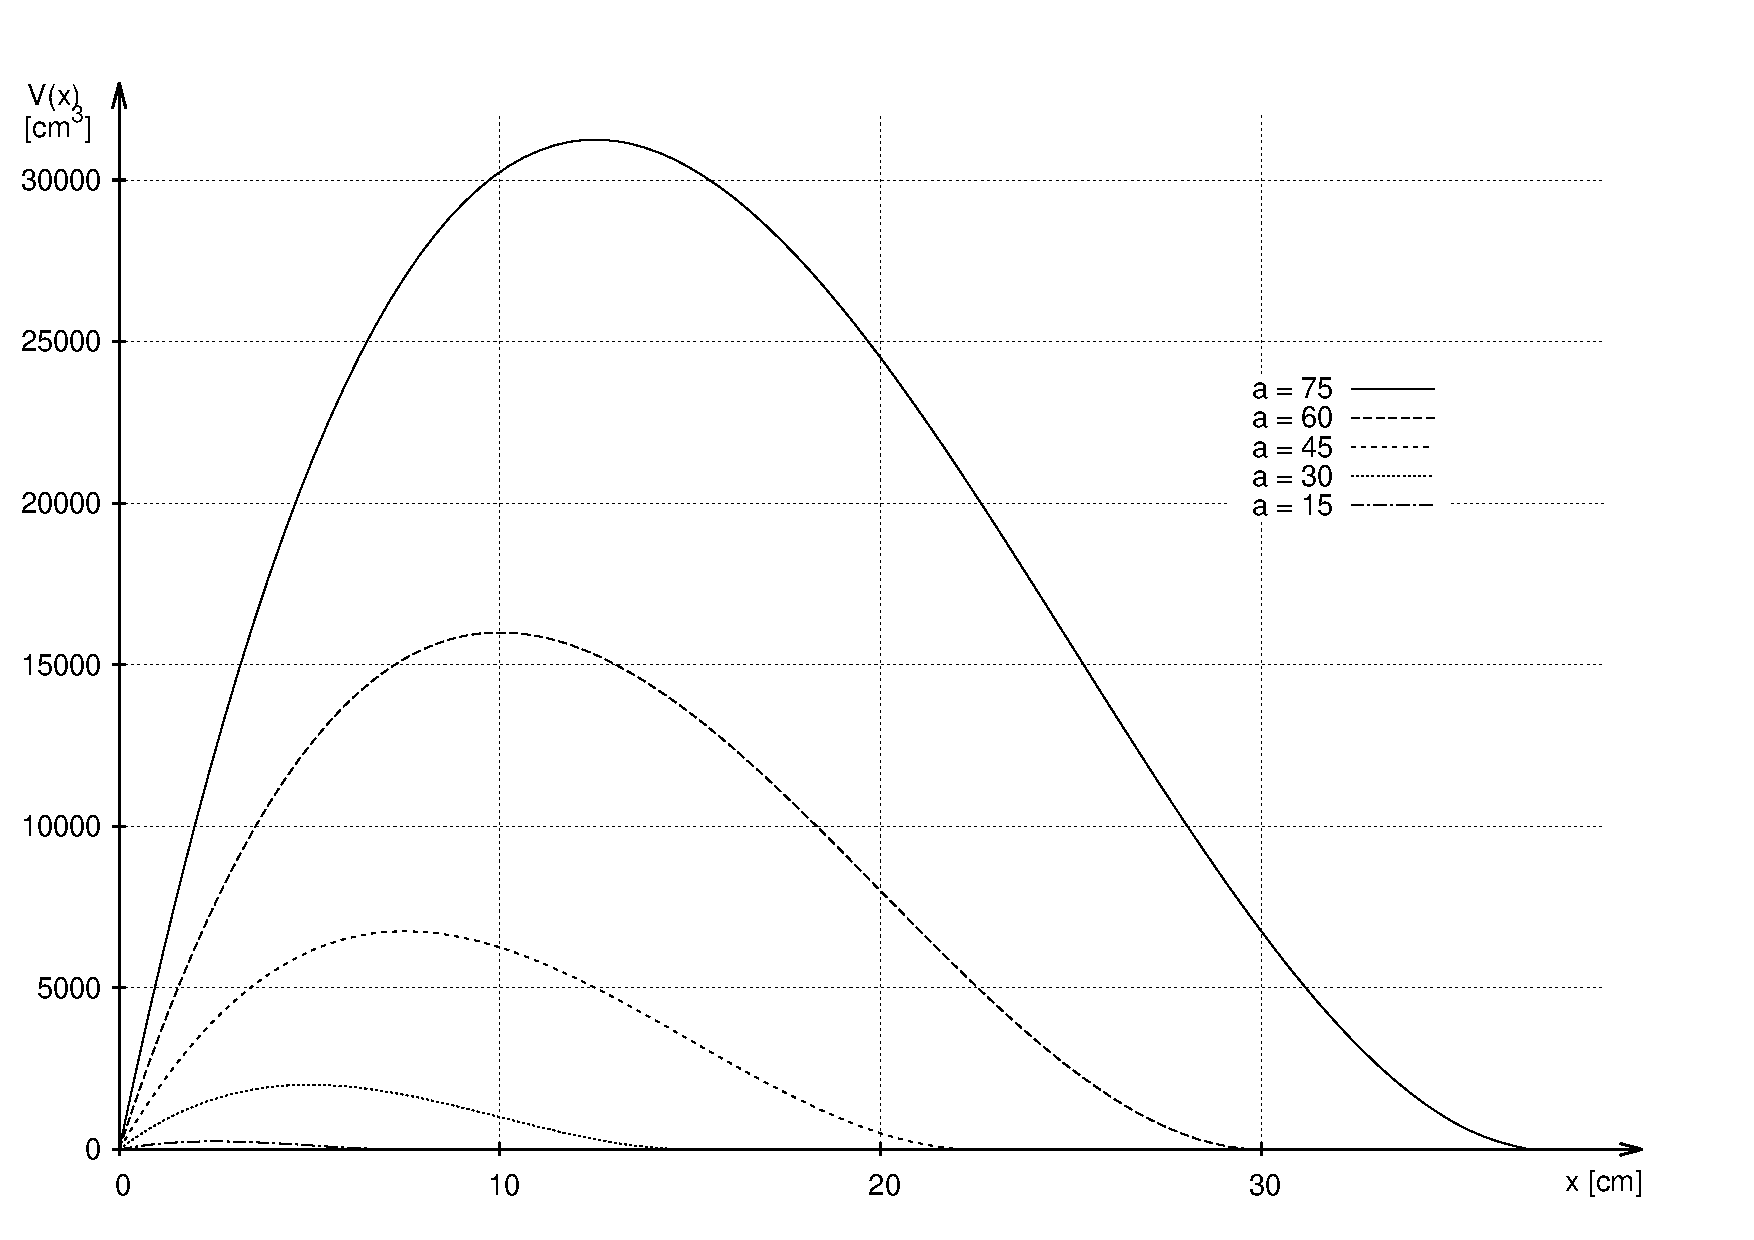
\includegraphics[width=0.8\linewidth]{pics/graph_1}
        
    \item Wir leiten  $ V_a(x)$ nach $x$ ab 
    $ V_a^\prime(x)=12x^2 - 8ax + a^2$ und bestimmen die Nullstellen
    (in Abhängigkeit von $a$): 
    $$12x^2 - 8ax + a^2=0
    \quad\Rightarrow\quad
    x^2 - \frac 2 3 a x + \frac 1 {12} a^2 = 0$$
    Für die Anwendung der p-q-Formel gilt nun: $p=- \frac 2 3 a$ und
    $q=\frac 1 {12} a^2$.
    Einsetzen in die p-q-Formel:
    $$x_{1,2}=\frac 1 3 a \pm \sqrt{\frac 1 9 a^2 - \frac 1 {12} a^2} 
    =\frac 1 3 a \pm \sqrt{\frac 1 {36} a^2} 
    = \frac 1 3 a \pm\frac 1 6 a 
    \quad \Rightarrow\quad x_1=\frac 1 2 a ;\quad x_2=\frac 1 6 a
    $$
    $x_1$ scheidet aus da $x<\frac a 2 $ gelten muss.

    Wir überprüfen $x_2$ mit der zweiten Ableitung:
    $ V_a^{\prime\prime}(x)=24x - 8a$
    $ V_a^{\prime\prime}(\frac 1 6 a)=24\frac 1 6 a - 8a = 4a-8a = -4a
    <0$, da $a>0$. Also liegt an der Stelle  $x_2=\frac 1 6 a$ ein
    Maximum vor. Die zweite Koordinate ermitteln wir durch Einsetzen
    der Stelle in die Funktion:
    $$V_a(\frac a 6)=4(\frac a 6)^3 - 4 a (\frac a 6)^2 + a^2\cdot
    \frac a 6=\frac 2 {27} a^3$$
    Also hat der Hochpunkt die Koordinaten: $H(\frac a 6|\frac 2 {27}a^3)$.
 
  \item Vergleichen Sie mit Ihren Klassenkolleginnen! 
  \end{enumerate}
\end{solution}
  Die $V_a$ mit $a\in\mathbb{R}$ bilden zusammen eine Schar. Jedes
  einzelne $V_a$ ist Mitglied der Schar. Das gleiche gilt für die
  Ableitungsfunktionen $V^\prime_a$. Auch sie bilden zusammen eine
  Schar. 
\newpage
  \subsection{Weitere Aufgaben}
  \begin{question}
    Wurfparabel

    Ein Fußball wird so geschossen, dass seine Flugbahn im Moment des Abschusses
    einen Winkel von $45^\circ$ nach oben einnimmt. Nun hängt es von der
    Geschwindigkeit des Balls ab, welche Bahn er beschreibt.

    Ist $v$ (in m/s) die Geschwindigkeit zum Zeitpunkt des Abschusses, dann
    kann die Flugbahn unter Vernachlässigung des Luftwiderstandes
    durch folgende Funktion beschrieben werden: 
    $$f_v(x)=-\frac 1 {v^2} \cdot 9,81\cdot x^2 + x$$
    Wobei die Koordinaten in der Maßeinheit m gemessen werden.
    Der Faktor 9,81 ist durch die jeweils wirkende
    Fallbeschleunigung zu ersetzen (Mond: 1,62). 

  \begin{enumerate}\itemsep0pt
  \item Zeichnen Sie die Wurfparabeln für die Geschwindigkeiten
    \begin{enumerate}
      \begin{multicols}{3}
      \item $6\,$m/s
      \item $9\,$m/s
      \item $12\,$m/s
      \end{multicols}
    \end{enumerate}
    in ein Koordinatensystem, dessen $x$-Achse von 0 bis 15 und dessen
    $y$-Achse von 0 bis 4 reicht. Abschusspunkt ist jeweils $(0|0)$. 
     \item Bestimmen Sie jeweils rechnerisch die Schussweite.
    \item Ermitteln Sie jeweils den höchsten Punkt der Flugbahn.
    \item \label{ball:v:30m}Bestimmen Sie die nötige
      Abschussgeschwindigkeit, um den Ball $30\,$m weit zu schießen.
    \item Berechnen Sie die Schussweite, die man erreichen könnte,
      wenn man den Ball mit der Abschussgeschwindigkeit aus
      \ref{ball:v:30m}.)  auf dem Mond schießen würde.
    \item Bestimmen Sie die Schussweite und den Scheitelpunkt der
      Flugbahn für alle $v\in\mathbb{R}^+$.
    \item Wie können Sie das letzte Ergebniss mit den vorigen in
      Einklang bringen?
    \item Bestimmen Sie die nötige Abschussgeschwindigkeit, damit der
      Ball $7\,$m hoch fliegt.
   \end{enumerate}
\end{question}
\begin{solution}
  \begin{enumerate}
  \item Flugbahnen für unterschiedliche Geschwindigkeiten.

    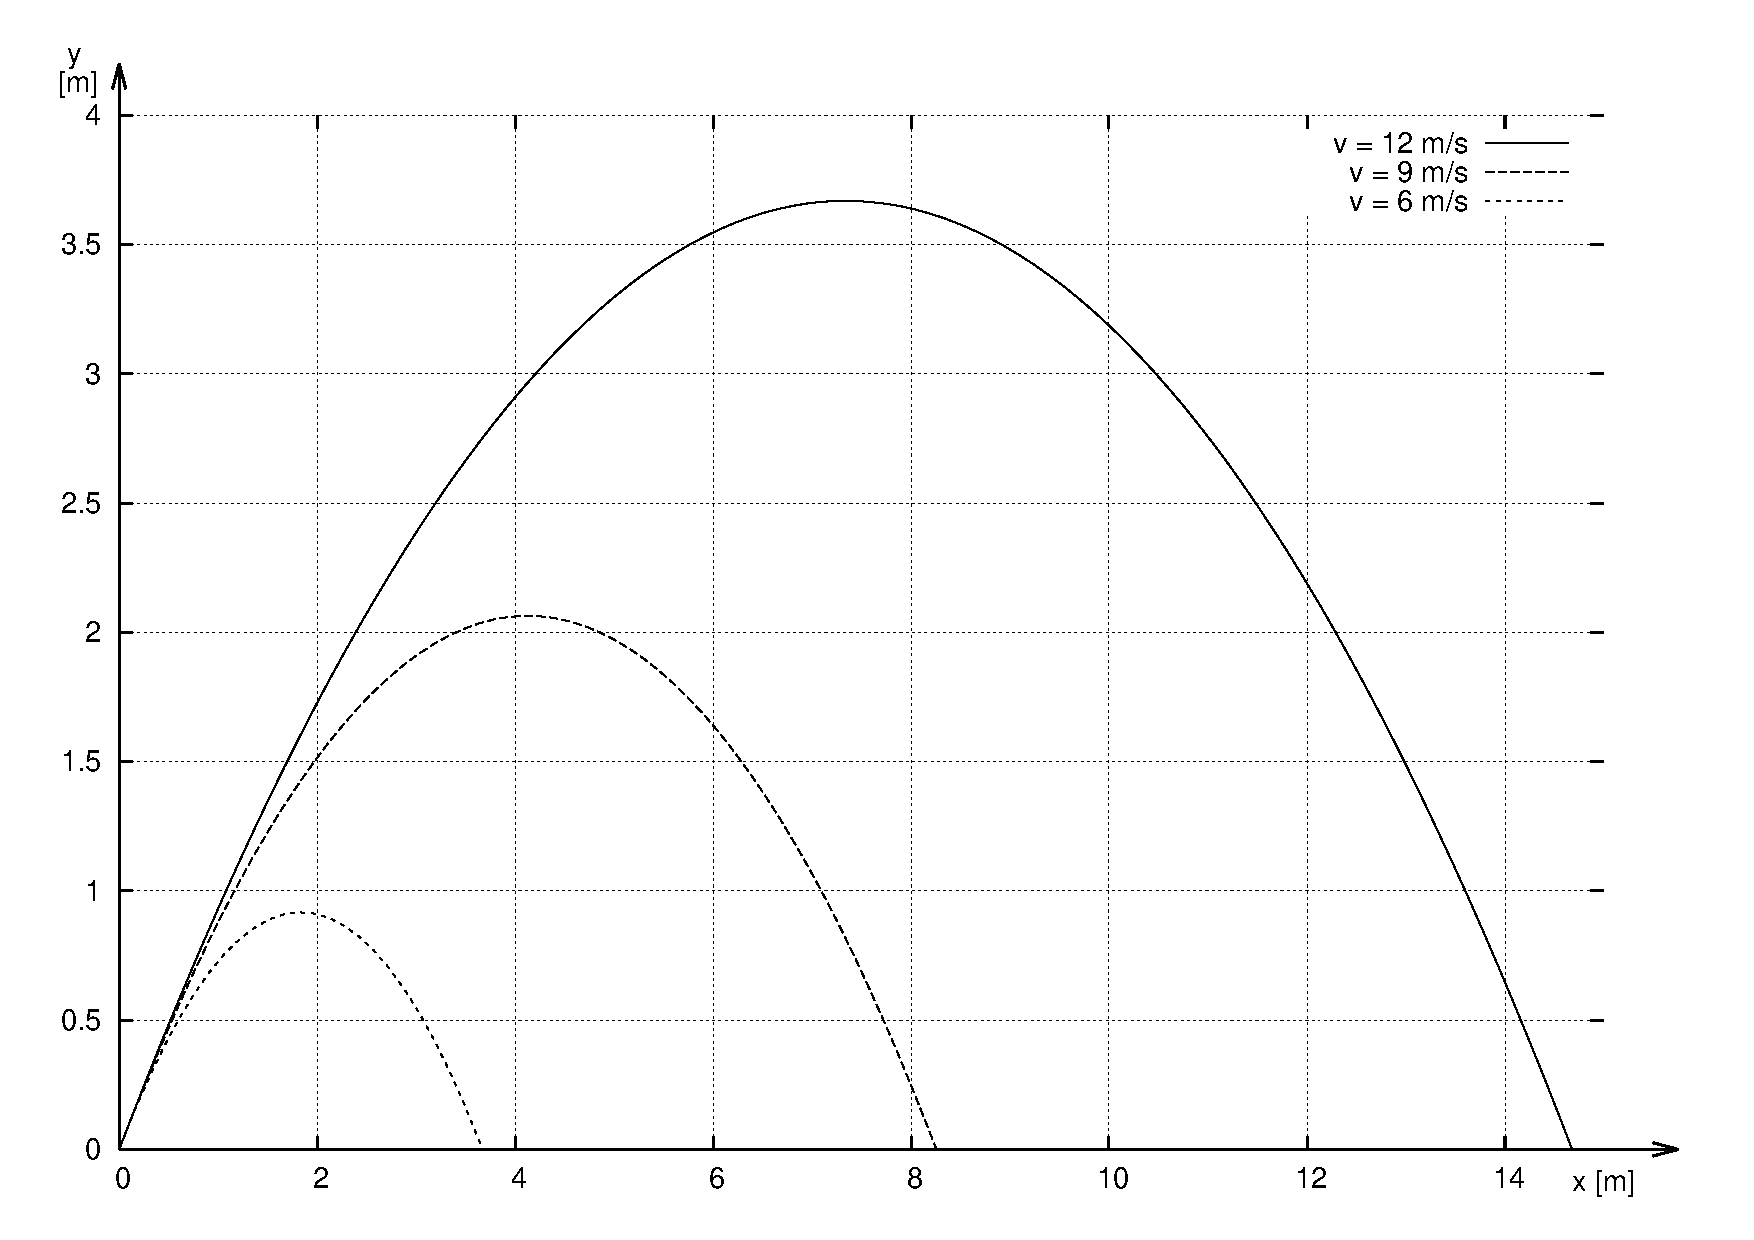
\includegraphics[width=.8\linewidth]{pics/graph_2}
  \item
    \begin{multicols}{3}
      \begin{enumerate}
      \item $3,669\,$m
      \item $8,257\,$m
      \item $14,679\,$m
      \end{enumerate}
    \end{multicols}
  \item
    \begin{multicols}{3}
      \begin{enumerate} 
      \item $H(1,835|0,917)$
      \item $H(4,128|2,064)$
      \item $H(7,339|3,67)$
      \end{enumerate}
    \end{multicols}
  \item Auf $f$ bezogen heißt die Forderung: $f$ hat bei $x=30$ eine
    Nullstelle. Man sucht das passende $v$. Also muss
    $-\frac 1 {v^2} \cdot 9,81\cdot 30^2 + 30=0$ nach $v$
    umgestellt werden. Man erhält:
    $v_{1,2}=\pm\sqrt{9,81\cdot 30}\approx \pm 17,1552\,$[m/s]. Da wir
    nur nach vorne schießen, entfällt die negative Lösung.
  \item Auf dem Mond gilt für die Flugbahn die Funktionsgleichung 
    $g_v(x)=-\frac 1 {v^2} \cdot 1,62\cdot x^2 + x$. Wir setzen die
    Geschwindigkeit $v=17,1552$ ein und ermitteln die Nullstellen der
    Funktion. Ihr Abstand voneinander beträgt $181,6672\,$m.
  \item Für die Schussweite bestimmen wir die zweite Nullstelle von
    $f$ in Abhängigkeit von $v$.
    $$f_v(x) \overset{!}{=} 0
    \quad \Rightarrow\quad 
    -\frac 1 {v^2} \cdot 9,81\cdot x^2 + x=0
    \quad \Rightarrow\quad 
    (-\frac 1 {v^2} \cdot 9,81\cdot x + 1)\cdot x=0
    \quad \Rightarrow\quad 
    -\frac 1 {v^2} \cdot 9,81\cdot x + 1 = 0 \textrm{ oder } x=0$$
    Für den ersten Term gilt dann:
    $$\frac {9,81} {v^2} \cdot x = 1 
    \quad\Rightarrow\quad
     x = \frac{v^2}{9,81} $$
     was der gesuchten Schussweite entspricht.
     Für den Scheitelpunkt betrachten wir:
     $$f^\prime_v(x)= - \frac 2 {v^2} \cdot 9,81 \cdot x + 1
     \textrm{ und }
     f^{\prime\prime}_v(x)= - \frac 2 {v^2} \cdot 9,81 <0$$
     Daraus ergibt sich für die Nullstelle der ersten Ableitung:
     $x_H= \frac {v^2}{ 2\cdot 9,81}$. Da die zweite Ableitung immer
     negativ ist, liegt ein Maximum vor. Für die $y$-Koordinate des
     Hochpunktes setzen wir $x_H$ in $f_v(x)$ ein:
     $$f_v(x_H)=y_H=
     -\frac 1 {v^2} \cdot 9,81\cdot 
     ( \frac {v^2}{ 2\cdot 9,81})^2 + \frac {v^2}{ 2\cdot 9,81} =
     -\frac {v^2}{4\cdot 9,81} +\frac {v^2}{ 2\cdot 9,81}
     = \frac {v^2}{ 4\cdot 9,81}
     $$
     Für die Koordinaten des Hochpunktes $H(x_H|y_H)$ gilt also:
     $$H\left(\frac {v^2}{ 2\cdot 9,81}\Big|\frac {v^2}{ 4\cdot 9,81}\right) $$
   \item Ersetzen Sie in den Ergebnissen das $v$ durch die jeweilige
     Geschwindigkeit und überprüfen Sie die Werte.
   \item Die zweite Koordinate des Hochpunktes muss $7$ betragen:
     $$\frac {v^2}{ 4\cdot 9,81} \overset{!}{=}7   
     \quad\Leftrightarrow\quad
     v^2 =7\cdot 4\cdot 9,81 = 274,68
     \quad\Rightarrow\quad
     v_{1,2}=\pm \sqrt{274,68}\approx\pm16,5735
     $$
     Da wir nur positive Geschwindigkeiten zulassen, ist
     $v=16,5735\,$m/s die gesuchte Lösung.
  \end{enumerate}
\end{solution}

\begin{question}

  Frischen Sie Ihr Wissen über Parabeln und ihre Gleichungen aus der
  11. Klasse auf. Erläutern Sie die Bedeutung der Koeffizienten in den
  verschiedenen Arten der Parabelgleichungen:
  $$f(x)=ax^2+bx+c;\quad f(x)=a(x-x_S)^2 + y_S;\quad
  f(x)=a(x-d)\cdot(x-e)$$
  Überlegen Sie in den folgenden Aufgaben, welche Merkmale der Parabel
  sich ändern, wenn man den Parameter $t\in\mathbb{R}^+$ verändert und
  welche sich 
  nicht verändern. Formen Sie gegebenfalls den Funktionsterm in eine
  Form um.
  \begin{enumerate}\itemsep0pt
    \begin{multicols}{2}
    \item $f_t(x)=-\frac 1 2 tx^2+9$
    \item $f_t(x)=(x-t)^2-t^2$
    \item $f_t(x)=\frac 1 3 (x-2)(x+t)$
    \item $f_t(x)=\frac 1 8 t x^2+tx+3$
    \end{multicols}
\end{enumerate}
\end{question}
\begin{solution}
   \begin{enumerate}
      \item Die Streckung der Parabel verändert sich entgegen $t$, der
      Scheitelpunkt und der $y$-Achsenschnitt bleiben konstant.
    \item Streckung bleibt konstant, der Scheitelpunkt ändert sich
      (aber wie?).
    \item Streckung ist konstant, eine Nullstelle verschiebt sich,
      damit auch der Scheitelpunkt.
    \item Der Scheitelpunkt wandert senkrecht  und die Streckung
      ändert sich, der $y$-Achsenabschnitt ist konstant.
  \end{enumerate}
\end{solution}



\begin{question}\label{scharen:tangente}
  
  Gegeben ist eine Funktionenschar $f_a$ mit $a\in\mathbb{R}^+$.
  Berechnen Sie die Steigung der Tangente an den Graphen von $f_a$ an
  der Stelle $x=0$. Bestimmen Sie $a$ so, dass diese Steigung den Wert
  $1$ annimmt.  
  \begin{multicols}{2}
    \begin{enumerate}\itemsep0pt
    \item $f_a(x)=ax^2+ax$
    \item $f_a(x)=ax^3+x^2-2ax$
    \item $f_a(x)=a^3x^3- ax$
    \item $f_a(x)=a^2x^3-3ax^2+a^2x-4$
    \item $f_a(x)=ax^3+3x^2-2x$
    \item $f_a(x)=2ax^3+2a^2x^2+a^2x$
    \end{enumerate}
  \end{multicols}
\end{question}
\begin{solution}
  \begin{multicols}{3}
    \begin{enumerate}
    \item $m=f^\prime_a(0)=a;\quad a=1$
    \item $m=-2a;\quad a=- \frac 1 2$
    \item $m=-a;\quad a=-1$
    \item $m=a^2;\quad a=\pm 1$
    \item $m=-2;\quad$ nicht möglich
    \item $m=a^2;\quad a=\pm 1$
    \end{enumerate}
  \end{multicols}
\end{solution}

\begin{question}
  
Bearbeiten Sie die Aufgaben aus Aufgabe \ref{scharen:tangente} und betrachten
Sie nicht die Stelle $x=0$, sondern nun die Stelle $x=1$ (oder etwas
schwieriger $x=2$).

Überlegen und diskutieren Sie, warum die Aufgabenstellung nun
schwieriger geworden ist. 

Welche Aufgabe ist für Sie nur mit Taschenrechner lösbar? 
\end{question}

\begin{question}
  
  Gegeben ist eine Schar von Funktionen $f_t$ mit
  $t\in\mathbb{R}^+$. Bestimmen Sie die Nullstellen der Funktionen in
  Abhängigkeit von $t$. Berechnen Sie die Fläche $A_t$, die der Graph von
  $f_t$ mit der $x$-Achse einschließt. Bestimmen Sie $t$ so, dass die
  Fläche 8 Flächeneinheiten groß ist.
  \begin{multicols}{3}
      \begin{enumerate}\itemsep0pt
      \item $f_t(x)=x^2-t^2$
      \item $f_t(x)=x^2-2tx$
      \item $f_t(x)=-x^2 + \frac 1 2 t^2x$
      \item $f_t(x)=x^4-tx^2$
      \item $f_t(x)=tx^2-t^2x$
      \item $f_t(x)=-x^3 + 4t^2x^2$
      \end{enumerate}
    \end{multicols}
  \end{question}
  \begin{solution} \begin{multicols}{2}
    \begin{enumerate}
    \item $x_1=t;\;x_2=-t$;\\
      $A_t=|\int_{-t}^tf_t(x)dx|=
      |[\frac 1 3 x^3 - t^2x]_{-t}^t|=
      |[\frac 1 3 t^3 - t^2\cdot t] - [\frac 1 3 (-t)^3 - t^2\cdot (-t)]|
      =|-\frac 4 3 t^3|=\frac 4 3 t^3$;\\
      $\frac 4 3 t^3\overset{!}{=}8 \quad\Rightarrow\quad
      t^3= 6 \quad\Rightarrow\quad
      t=\sqrt[3]{6}\approx 1,8171$
    \item $x_1=0;\; x_2=2t;\quad A_t=\frac {4} 3 t^3;\quad
      t=\sqrt[3]{6}\approx 1,8171$
    \item $x_1=0;\; x_2=\frac 1 2 t^2; \quad A_t=\frac 1 {48} t^6; \quad
      t=\sqrt[6]{384}\approx 2,696$
    \item $x_1=0;\; x_2=\sqrt{t};\; x_3=-\sqrt{t};\\
      A_t=-\int_{-\sqrt{t}}^{\sqrt{t}}f_t(x)dx=
      \frac 4 {15}t^{\frac 5 2}=\frac 4 {15}\sqrt{t^5};\\
      t=\sqrt[5]{900}\approx 3,898$
    \item $x_1=0;\;x_2=t;\quad
      A_t=\frac 1 6 t^4;\quad
      t=\sqrt[4]{48}\approx 2,6321$
    \item $x_1=0;\;x_2=4t^2;\quad
      A_t=\frac{64} 3 t^8;\quad
      t=\sqrt[8]{\frac 3 8}\approx 0,88461$
    \end{enumerate}
  \end{multicols}
\end{solution}
  
\section{Ortskurven}
Verändert man den Parameter einer Funktionenschar, so verändern sich
die Funktionen und mit ihnen die Graphen in der Regel\footnote{Stimmt
  natürlich so nicht, aber bei den Scharen und Funktionen, die wir
  betrachten ist das in der Regel so.}  \emph{stetig}, das
heißt ohne Sprünge. Betrachten Sie dazu z. B. einen Hochpunkt eines
Graphen (z. B. den Scheitelpunkt aus der Aufgabe mit den
Wurfparabeln). Wenn Sie den Parameter ändern, wandert auch der
Hochpunkt und beschreibt dabei eine bestimmte Kurve -- seine
Ortskurve.
\subsection{Bestimmung von Ortskurven}
Betrachten Sie den Hochpunkt des Volumens aus dem Schachtelproblem:
$$H\left(\frac a 6\mid\frac 2 {27}a^3\right)$$ %%%Mittelstrich anpassen
Sie sehen, die Koordinaten sind vom Parameter $a$ -- der Seitenlänge
des Quadrats -- abhängig.

Stellen Sie die Veränderung der Lage des Hochpunktes in Abhängigkeit
von $a$ in einem Koordinatensystem dar. Überlegen Sie sich vorher,
welche Maße das Koordinatensystem haben muss und welche Quadranten
überhaupt benötigt werden. Es gelte dabei $1\leq a\leq 30$. 

Welcher Art ist die Kurve die alle Hochpunkte zusammen bilden?
Vergleichen Sie mit Ihren Kollegen.

Um eine mathematische Beschreibung für die Ortskurve zu bekommen,
wenden wir folgendes Verfahren an: 
Für die Koordinaten des Hochpunktes $H$ gilt: $x= \frac a 6$ und
$y=\frac 2 {27}a^3$. Wir stellen $x$ nach $a$ um: $a=6x$ und setzen
das $a$ nun in die Gleichung von $y$ ein: $y=\frac 2 {27}\cdot (6x)^3$
und vereinfachen zu $y=16x^3$ (Bitte rechnen Sie nach!).

Also liegen alle Hochpunkte auf dem Graphen der Funktion $f(x)=16x^3$.

\begin{question}

  Berechnen Sie die Ortskurve des Scheitelpunktes der Flugparabeln aus Aufgabe 2 6.).
\end{question}
\begin{solution}
  Da in beiden Koordinaten der Parameter im Quadrat steht, braucht man die quadratische Gleichung
  nicht zu lösen und kann direkt $v^2$ einsetzen. Wir erhalten dann für die Ortskurve: $y=\frac x 2$.
\end{solution}


\begin{question}
  Bestimmen Sie die Extrempunkte und die Ortskurven der Extrema der
  Funktionenscharen $f_t$.
  \begin{multicols}{2}
    \begin{enumerate}\itemsep0pt
    \item $f_t(x)=x^2-2tx;\quad t\in\mathbb{R}$
    \item $f_t(x)=x^2+tx-2x-2t;\quad t\in\mathbb{R}$
    \item $f_t(x)=\frac 1 8 tx^2+x+2;\quad t\in\mathbb{R}^+$
    \item $f_t(x)=x^3-t^2x;\quad t\in\mathbb{R}$
    \end{enumerate}
  \end{multicols}
\end{question}
\begin{solution}
  \begin{multicols}{2}
    \begin{enumerate}
    \item $H(t|-t^2);\;y=-x^2$
    \item $T(1-\frac t 2|-\frac {t^2} 4 -t -1);\; y=-x^2+4x-4$
    \item $T(-\frac 4 t|-\frac 2 t+2);\; y=\frac x 2 +2$ (Tipp: nach
      $\frac 2 t$ umstellen, da man nicht durch $x$ teilen darf!)
      \item $E_1(\frac t {\sqrt{3}}|-\frac{2t^3}{3\sqrt{3}}); 
             E_2(-\frac t {\sqrt{3}} | \frac{2t^3}{3\sqrt{3}});$
             Beide Extrema liegen auf der gleichen Ortskurve:
             $y=-2x^3$.
    \end{enumerate}
  \end{multicols}
\end{solution}

\section{Fixpunkte}
\begin{minipage}[b]{0.39\linewidth}
  In der Abbildung sind die Graphen einiger Funktionen der Schar
$$f_a(x)=\frac 1 5 x^3 -\frac 1 2 ax^2 +x+5a;\quad a\in\mathbb{R}^+$$
dargestellt.

Es ist leicht zu sehen, dass alle Mitglieder dieser Schar zwei
gemeinsame Punkte haben. Nicht alle Scharen haben gemeinsame Punkte,
sogenannte Fixpunkte. 

\vspace{1cm}

\end{minipage}
\hfill
\begin{minipage}[b]{0.6\linewidth}
  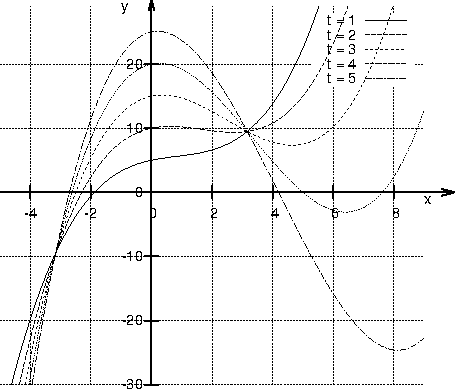
\includegraphics[width=1\linewidth]{pics/graph_3}
\end{minipage}
\subsection{Bestimmung von Fixpunkten}
Um die Fixpunkte einer Schar zu bestimmen, muss man folgende Gleichung
lösen:
$$f_a(x)=f_b(x)\quad \textrm{mit } a\neq b$$
Versuchen Sie die Fixpunkte der obigen Schar zu bestimmen, ehe Sie
weiter lesen.

Dem obigen Ansatz folgend erhält man die Gleichung: 
$$\frac 1 5 x^3 -\frac 1 2 ax^2 +x+5a 
=
\frac 1 5 x^3 -\frac 1 2 bx^2+x+5b$$
Wir ziehen $\frac 1 5 x^3$ und $x$ auf beiden Seiten ab und erhalten:
$$-\frac 1 2 ax^2+5a = -\frac 1 2 bx^2+5b$$
Wir stellen alle Terme mit $x$ nach links, die konstanten nach rechts:
$$\frac 1 2 bx^2-\frac 1 2 ax^2 = 5b-5a$$
Dann klammern wir $b-a$ aus (das ist quasi der Hauptschritt):
$\frac 1 2 x^2 (b-a) = 5(b-a)$.
Da $b\neq a$, ist $b-a\neq 0$ und wir dürfen durch $b-a$ teilen:
$\frac 1 2 x^2= 5$.
Wir lösen die quadratische Gleichung und erhalten als Lösungen:
$x_1=\sqrt{10};\; x_2=-\sqrt{10}$. Es bleibt nur noch, die Werte in
$f_a$ einzusetzen (dabei wählen wir ein möglichst bequemes $a$) um die
$y$-Werte der Fixpunkte zu bekommen und erhalten:
$F_1(-\sqrt{10}|-3\sqrt{10})$ und $F_2(\sqrt{10}|3\sqrt{10})$.
\begin{question}

  Bestimmen Sie die gemeinsamen Punkte der folgenden Scharen.
  \begin{enumerate}
    \begin{multicols}{2}
    \item $f_a(x)=ax^2+2ax-3a;\;a\in\mathbb{R}$
    \item $f_a(x)=ax^2-4ax+4a+4;\;a\in\mathbb{R}$
    \item $f_a(x)=x^3-ax^2-4x+4a;\;a\in\mathbb{R}$
    \item $f_a(x) = x^3 + a x^2 - a x + 4;\;a\in\mathbb{R}$
    \end{multicols}
  \item $f_a(x)=x^3-4x^2-ax^2+4ax-21x+21a+8;\;a\in\mathbb{R}$
  \end{enumerate}
\end{question}
\begin{solution}
   \begin{enumerate}
    \begin{multicols}{3}
    \item $F_1(1|0);\;F_2(-3|0)$
    \item $F(2|4)$
    \item $F_1(2|0);\;F_2(-2|0)$
    \item $F_1(0|4);\;F_2(1|5)$
    \item $F_1(-3|8);\;F_2(7|8)$
    \end{multicols}
  \end{enumerate}
\end{solution}
\section{Übungsaufgaben}
\begin{question}
  Springbrunnen

An der Längsseite eines 20\,m langen und 3\,m breiten Wasserbeckens
sind die Düsen so angebracht, dass die Wasserfontänen im rechten Winkel
zum Rand aufsteigen, eine Parabel beschreiben und dann im Becken auf
das Wasser auftreffen. Dabei kann die Parabel in Abhängigkeit vom
Wasserdruck durch folgende Gleichung modelliert werden:
$$f_t(x)=4x^2+\frac 1 2 tx;\quad t\in\mathbb{R}^+$$
Dabei sind alle Angaben in Metern und die Düse befindet sich im
Ursprung.
\begin{enumerate}
\item Skizzieren Sie den Sachverhalt in einem Koordinatensystem.
\item Zeichnen Sie die Fontänen für die Parameter $t=8$ und $t=12$ in
  die Skizze ein.
\item Bestimmen Sie den Parameter so, dass die Fontäne 1\,m von der
  Düse entfernt auftrifft.
\item Bestimmen Sie den maximalen Wert für $t$, so dass die Fontäne
  noch im Becken auftrifft. Ermitteln Sie die Höhe, die die Fontäne
  dann erreicht.
\item Für welchen Wert von $t$ erreicht die Fontäne eine Höhe von
  4\,m? Wie weit von der Düse entfernt trifft die Fontäne dann auf?
\item Bestimmen Sie die Ortskurve des Scheitelpunktes.
\item Bestimmen Sie alle gemeinsamen Punkte der Fontänen.
\end{enumerate}

\end{question}
\begin{solution}
  \begin{enumerate}
    \begin{minipage}[t]{0.4\linewidth}
    \item
      Graph der Fontäne für verschiedene Parameter

      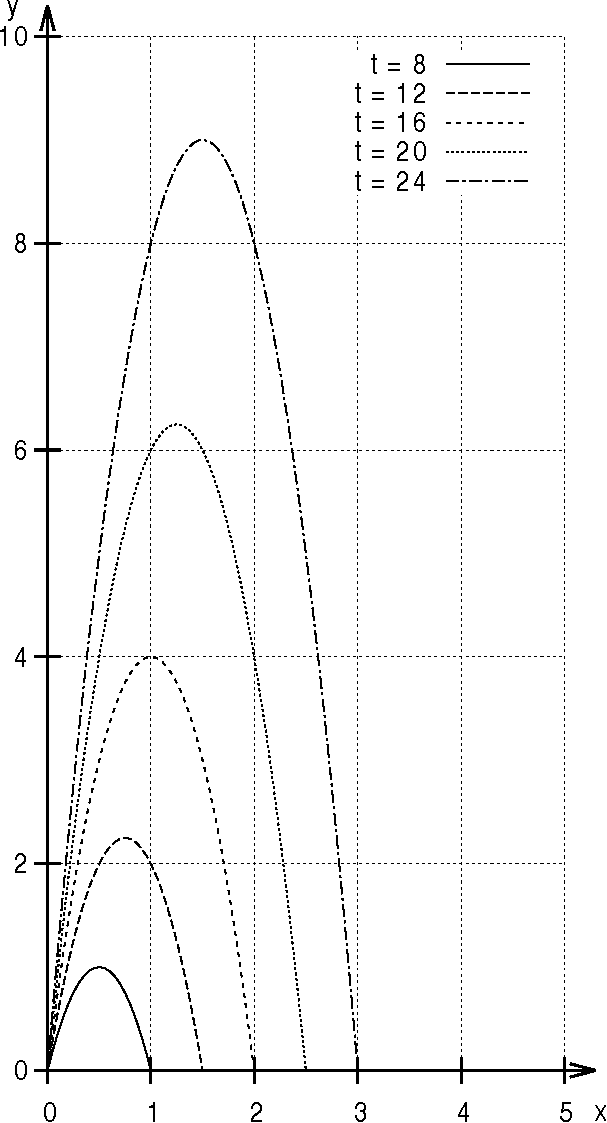
\includegraphics[width=\linewidth]{pics/graph_4_1}
    \end{minipage}
    \hfill
\setcounter{enumi}{2}
\begin{minipage}[t]{0.5\linewidth}
\item $t=8$
\item $t=24$; $S(1,5|9)$
\item $t=16$; 2\,m
\item $S(\frac t {16}| \frac {t^2} {64})$;\; $y_S=4x^2$
\item $F(0|0)$
\end{minipage}
\end{enumerate}
\end{solution}

\newpage
\section{Lösungen der Aufgaben}
{\scriptsize\printsolutions}
\end{document}


